\documentclass[12pt,a4paper]{article}

\usepackage[utf8]{inputenc}
\usepackage[T1]{fontenc}
\usepackage[brazil]{babel}
\usepackage{lmodern}
\usepackage{geometry}
\usepackage{graphicx}
\usepackage{booktabs}
\usepackage{longtable}
\usepackage{array}
\usepackage{pdflscape}
\usepackage{caption}
\usepackage{subcaption}
\usepackage{float}
\usepackage{hyperref}
\usepackage{xcolor}
\usepackage{adjustbox}

\geometry{
  left=3cm,
  right=2cm,
  top=3cm,
  bottom=2cm
}

\hypersetup{
  colorlinks=true,
  linkcolor=black,
  urlcolor=black,
  citecolor=black
}

\graphicspath{{figuras/}{figuras/gantt/}{dashboard/}{tabelas/}}
\setlength{\parindent}{1.25cm}
\setlength{\parskip}{0.2em}
\renewcommand{\arraystretch}{1.15}

% Campos editáveis da capa.
\newcommand{\universidade}{Universidade Federal do Amazonas}
\newcommand{\curso}{Curso}
\newcommand{\disciplina}{Disciplina}
\newcommand{\professor}{Professor}
\newcommand{\autora}{Tárcila Jéssica Silva de Sousa}
\newcommand{\matricula}{Matrícula}
\newcommand{\titulo}{Análise Computacional de Problemas de Escalonamento}
\newcommand{\subtitulo}{Machine Scheduling, Job Shop Scheduling e Flow Shop}
\newcommand{\localidade}{Manaus}
\newcommand{\ano}{2026}

\begin{document}

\begin{titlepage}
  \centering
  {\large \universidade\par}
  \vspace{0.5cm}
  {\large \curso\par}
  {\large \disciplina\par}
  \vspace{0.5cm}
  {\large Professor(a): \professor\par}

  \vfill

  {\large \autora\par}
  {\large Matrícula: \matricula\par}

  \vfill

  {\bfseries\Large \titulo\par}
  \vspace{0.4cm}
  {\large \subtitulo\par}

  \vfill

  {\large \localidade\par}
  {\large \ano\par}
\end{titlepage}

\pagenumbering{arabic}

\section{Resultados}

Esta seção apresenta os resultados computacionais consolidados a partir dos
arquivos gerados nos experimentos. Foram considerados apenas os valores
registrados em \texttt{resultados\_completos.csv}, nas tabelas derivadas desse
arquivo e nos dados detalhados utilizados para os gráficos de Gantt.

\subsection{Visão geral das execuções}

A Tabela~\ref{tab:geral} resume os resultados por problema. O conjunto contém
48 instâncias, das quais 29 foram registradas com status ótimo. Não houve erros
nos resultados consolidados.

\begin{table}[H]
\centering
\caption{Resumo geral dos experimentos por problema.}
\label{tab:geral}
\scriptsize
\begin{adjustbox}{max width=\textwidth}
\begin{tabular}{lrrrrrrrrrrrrrr}
\toprule
Problema & Inst. & Ótimas & Viáv. não ót. & Lim. tempo & Erros &
Tempo méd. & Tempo med. & Maior tempo & Gap méd. & Maior gap &
Tarefas méd. & Máq. méd. & Var. méd. & Restr. méd. \\
\midrule
Machine Scheduling & 31 & 17 & 14 & 14 & 0 & 150,670 & 119,012 & 300,019 & 0,3841 & 1,0000 & 13,871 & 1,000 & 148,548 & 445,645 \\
Job Shop Scheduling & 10 & 6 & 4 & 4 & 0 & 190,464 & 235,695 & 300,218 & 0,1297 & 0,6008 & 10,600 & 7,100 & 448,600 & 1344,800 \\
Flow Shop Scheduling & 7 & 6 & 1 & 1 & 0 & 44,178 & 0,619 & 300,249 & 0,0079 & 0,0241 & 17,143 & 5,571 & 439,571 & 741,286 \\
\bottomrule
\end{tabular}
\end{adjustbox}
\end{table}

Observa-se que Flow Shop Scheduling apresentou a maior proporção de resultados
ótimos, enquanto Job Shop Scheduling apresentou os maiores tempos médio e
mediano. Machine Scheduling concentrou o maior número absoluto de limites de
tempo e o maior gap médio.

\begin{figure}[H]
\centering
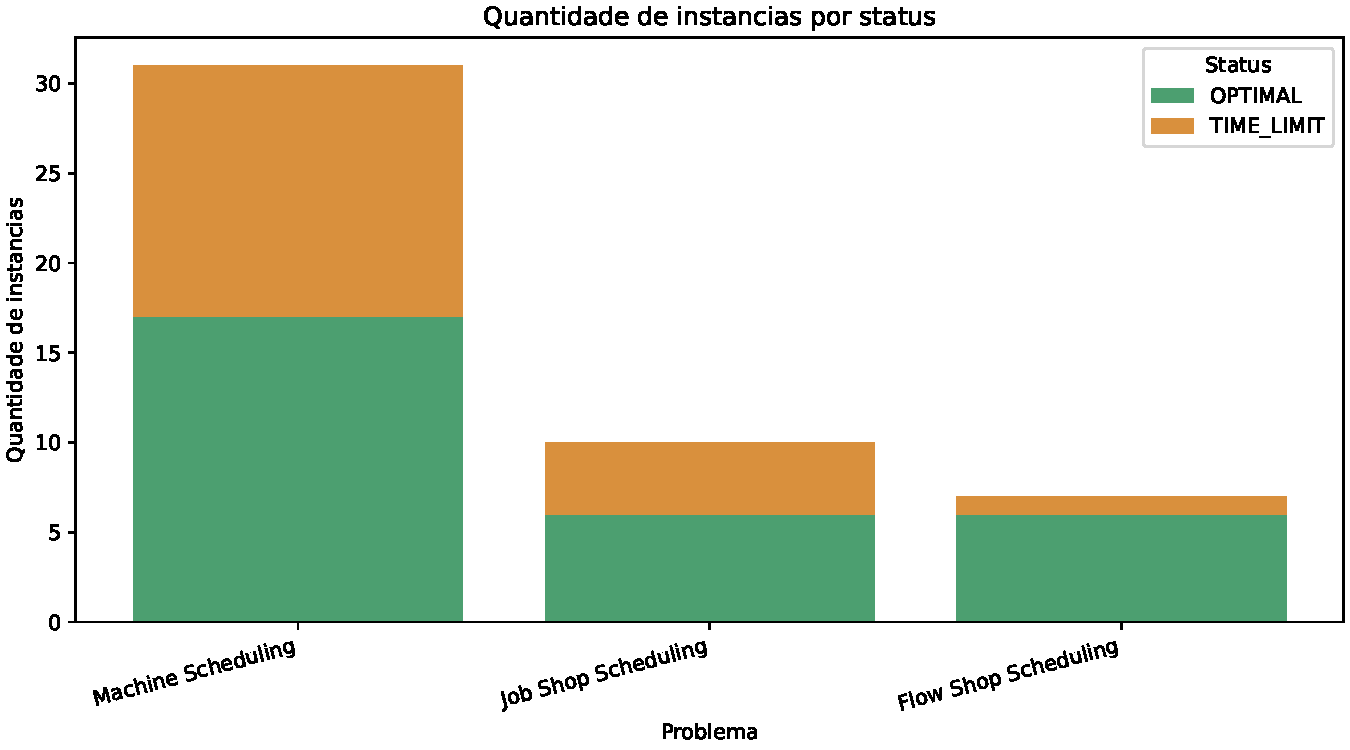
\includegraphics[width=0.92\textwidth]{quantidade_instancias_por_status.pdf}
\caption{Quantidade de instâncias por status de terminação.}
\label{fig:status}
\end{figure}

A Figura~\ref{fig:status} mostra que os três problemas tiveram instâncias
resolvidas com status ótimo e instâncias interrompidas pelo limite de tempo. O
número absoluto de interrupções foi maior em Machine Scheduling.

\begin{figure}[H]
\centering
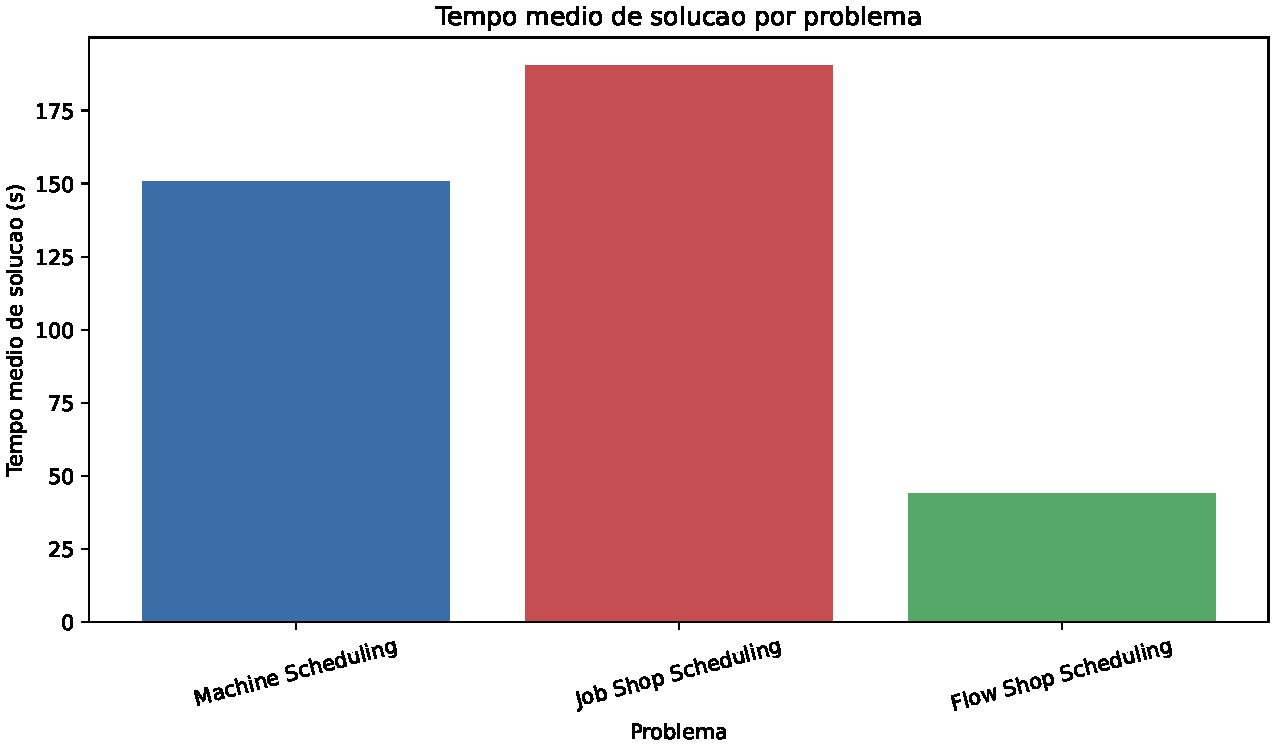
\includegraphics[width=0.86\textwidth]{tempo_medio_por_problema.pdf}
\caption{Tempo médio de solução por problema.}
\label{fig:tempo-medio}
\end{figure}

A Figura~\ref{fig:tempo-medio} evidencia a diferença de tempo médio entre os
problemas. Job Shop Scheduling apresentou o maior tempo médio, seguido por
Machine Scheduling e Flow Shop Scheduling.

\subsection{Machine Scheduling}

Machine Scheduling teve 31 instâncias analisadas, com 17 resultados ótimos, 14
soluções viáveis não ótimas e 14 interrupções por limite de tempo. Como as
instâncias possuem uma máquina, o crescimento do número de tarefas concentrou a
dificuldade nas decisões de sequenciamento.

\begin{figure}[H]
\centering
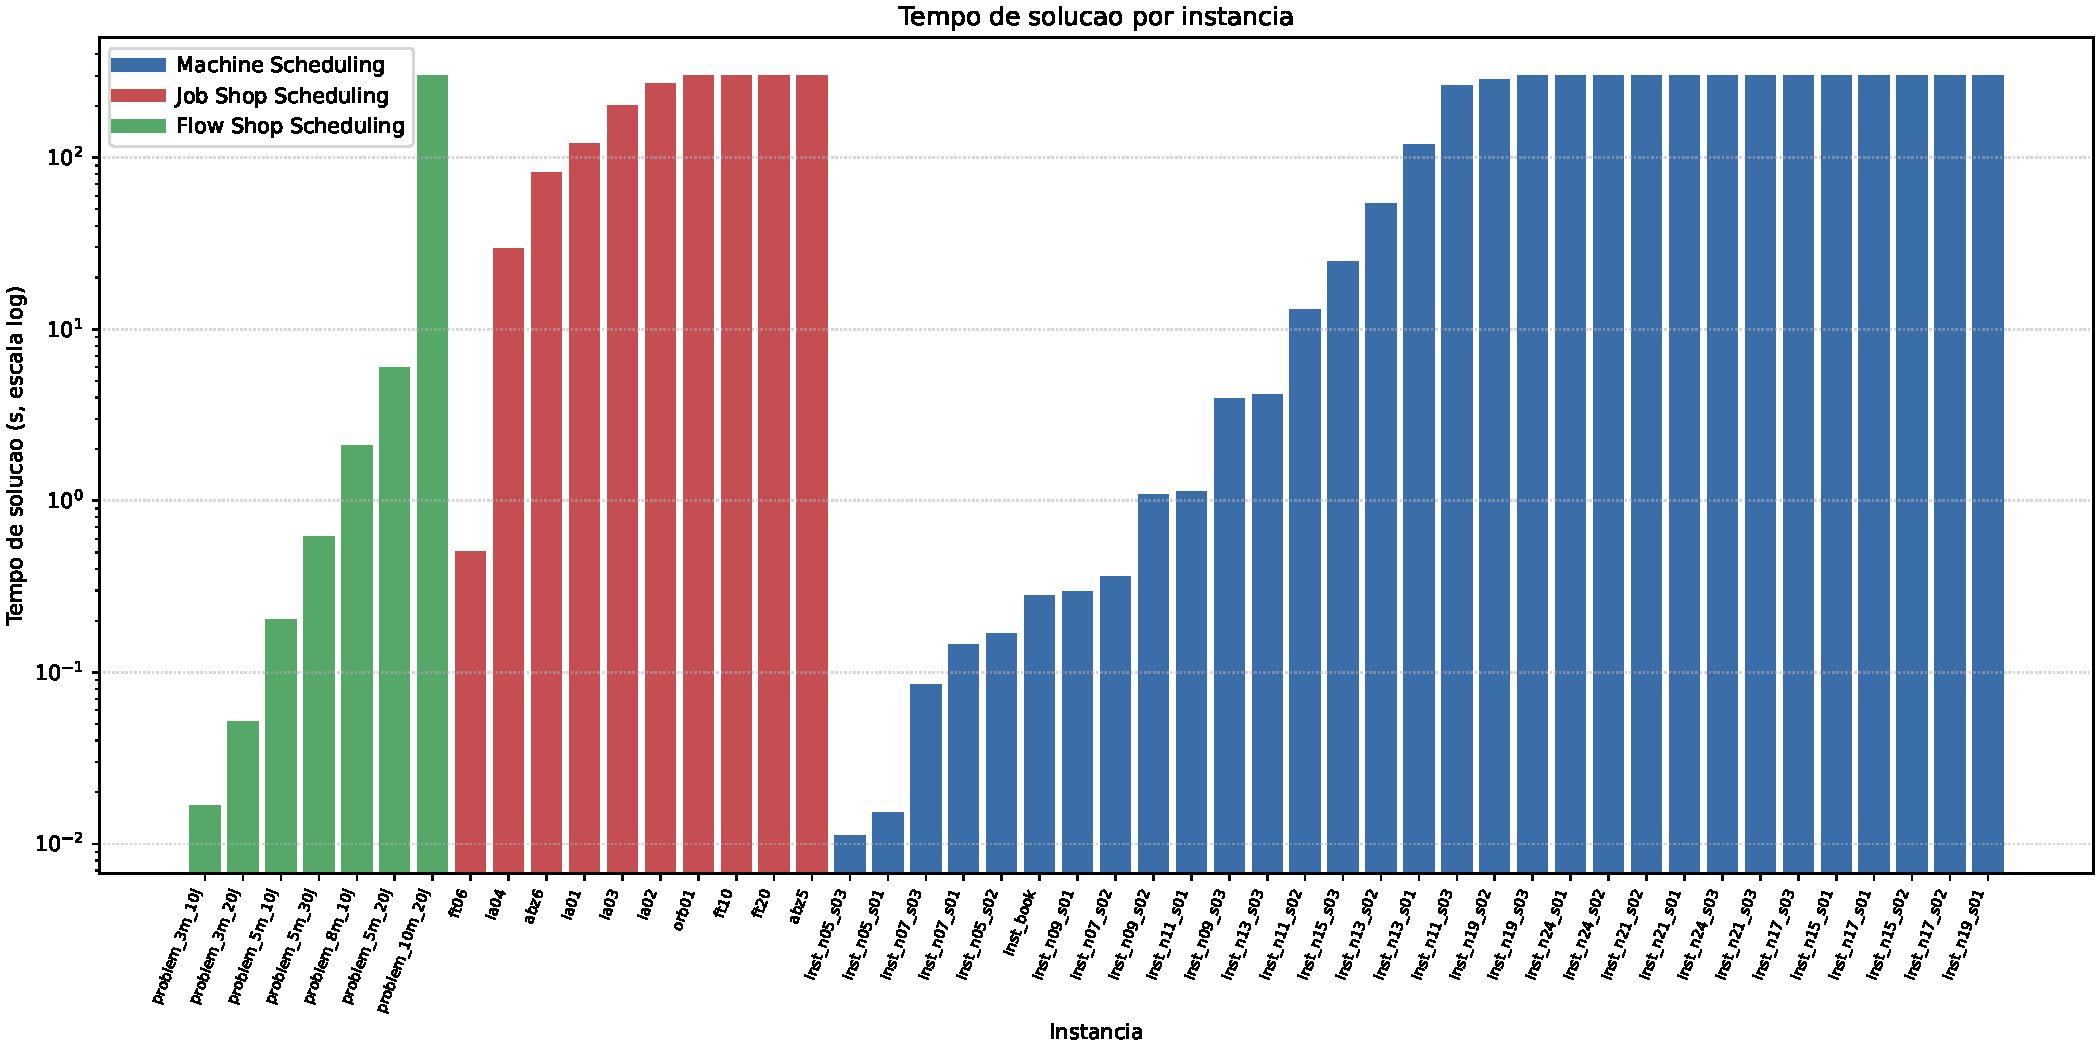
\includegraphics[width=0.95\textwidth]{tempo_solucao_por_instancia.pdf}
\caption{Tempo de solução por instância.}
\label{fig:tempo-instancia}
\end{figure}

Na Figura~\ref{fig:tempo-instancia}, as instâncias de Machine Scheduling de
maior porte aparecem frequentemente próximas ao limite de 300 segundos,
indicando dificuldade para encerrar a resolução dentro da tolerância
configurada.

\begin{figure}[H]
\centering
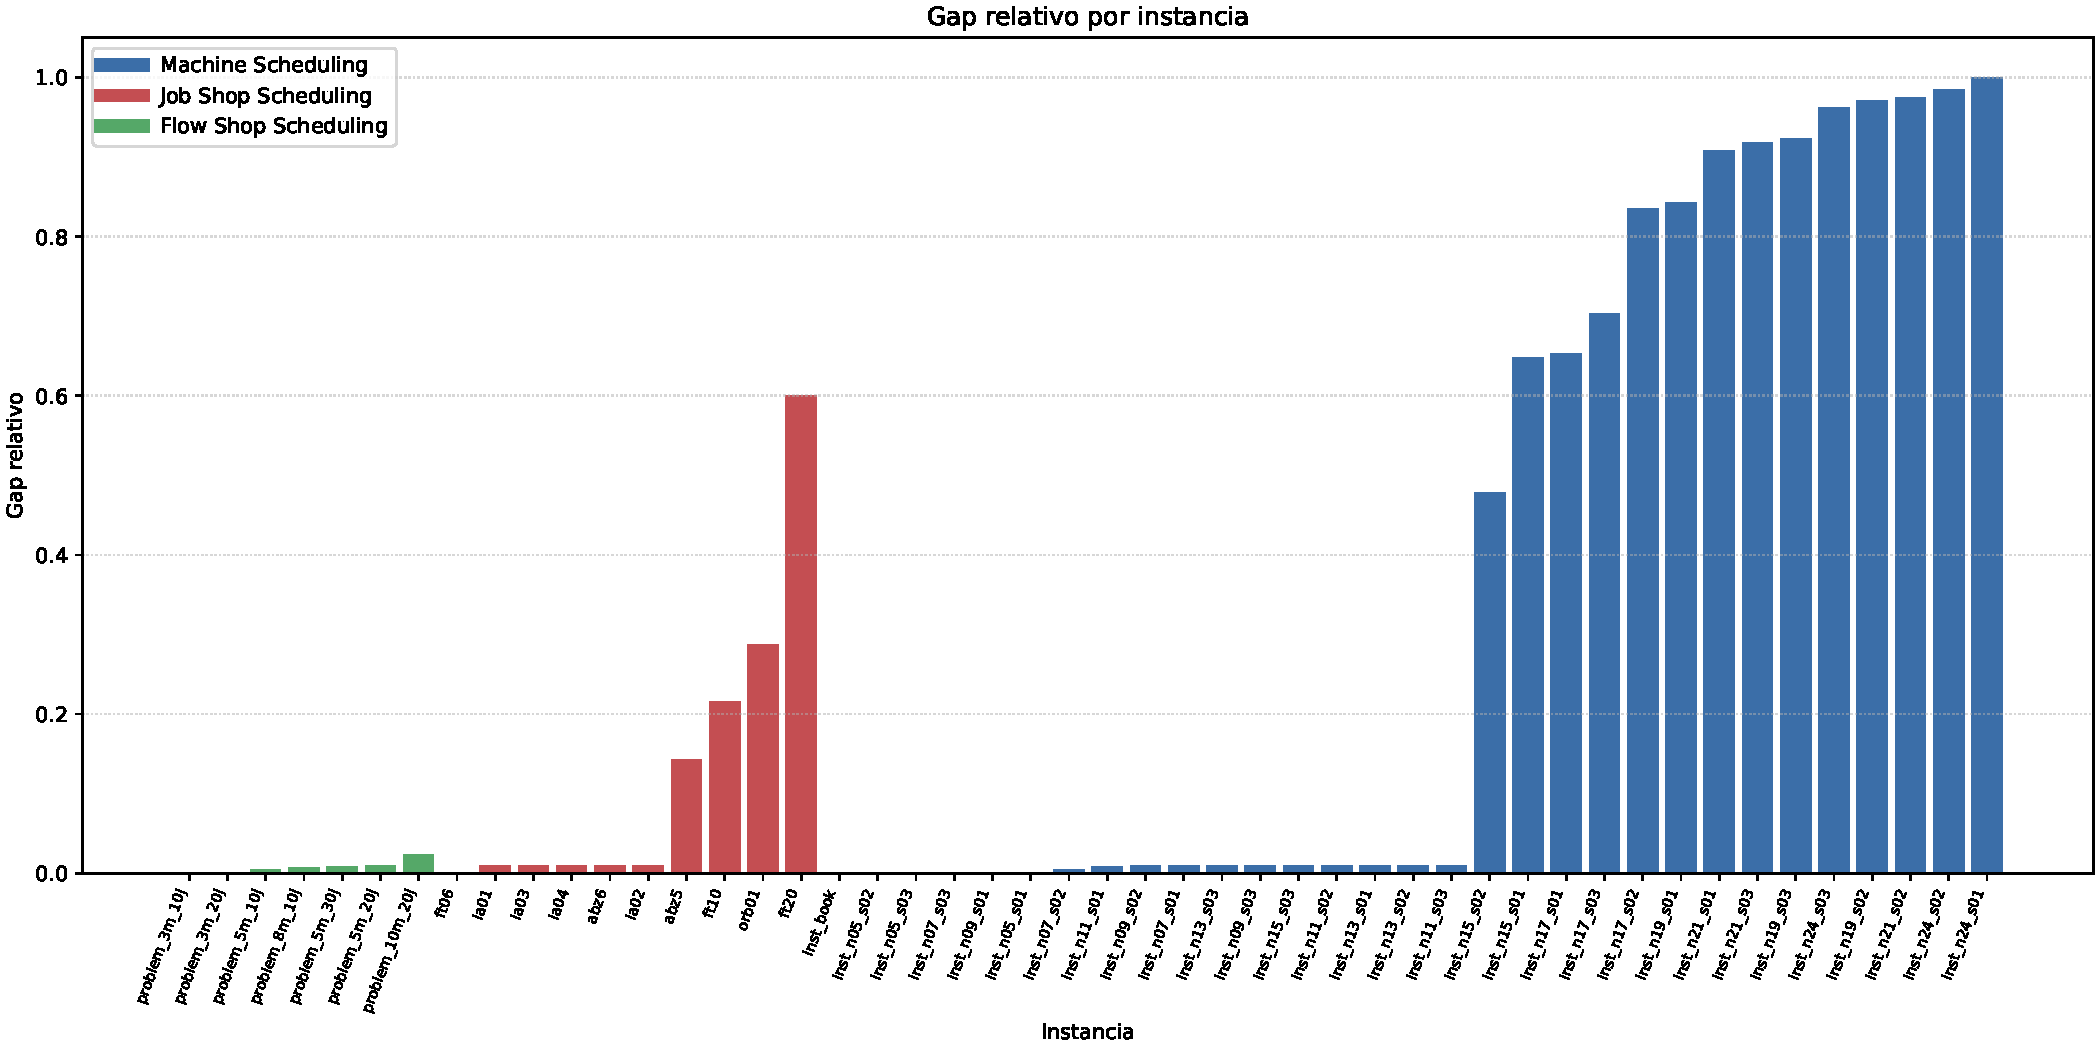
\includegraphics[width=0.90\textwidth]{gap_por_instancia.pdf}
\caption{Gap relativo por instância.}
\label{fig:gap-instancia}
\end{figure}

A Figura~\ref{fig:gap-instancia} mostra que os maiores gaps foram observados em
Machine Scheduling. Esse comportamento é coerente com os resultados da
Tabela~\ref{tab:geral}, em que esse problema apresentou o maior gap médio e o
maior gap máximo.

\subsection{Job Shop Scheduling}

Job Shop Scheduling teve 10 instâncias analisadas, com 6 resultados ótimos e 4
interrupções por limite de tempo. O problema apresentou os maiores tempos médio
e mediano, o que indica maior esforço computacional central no conjunto
avaliado.

\begin{figure}[H]
\centering
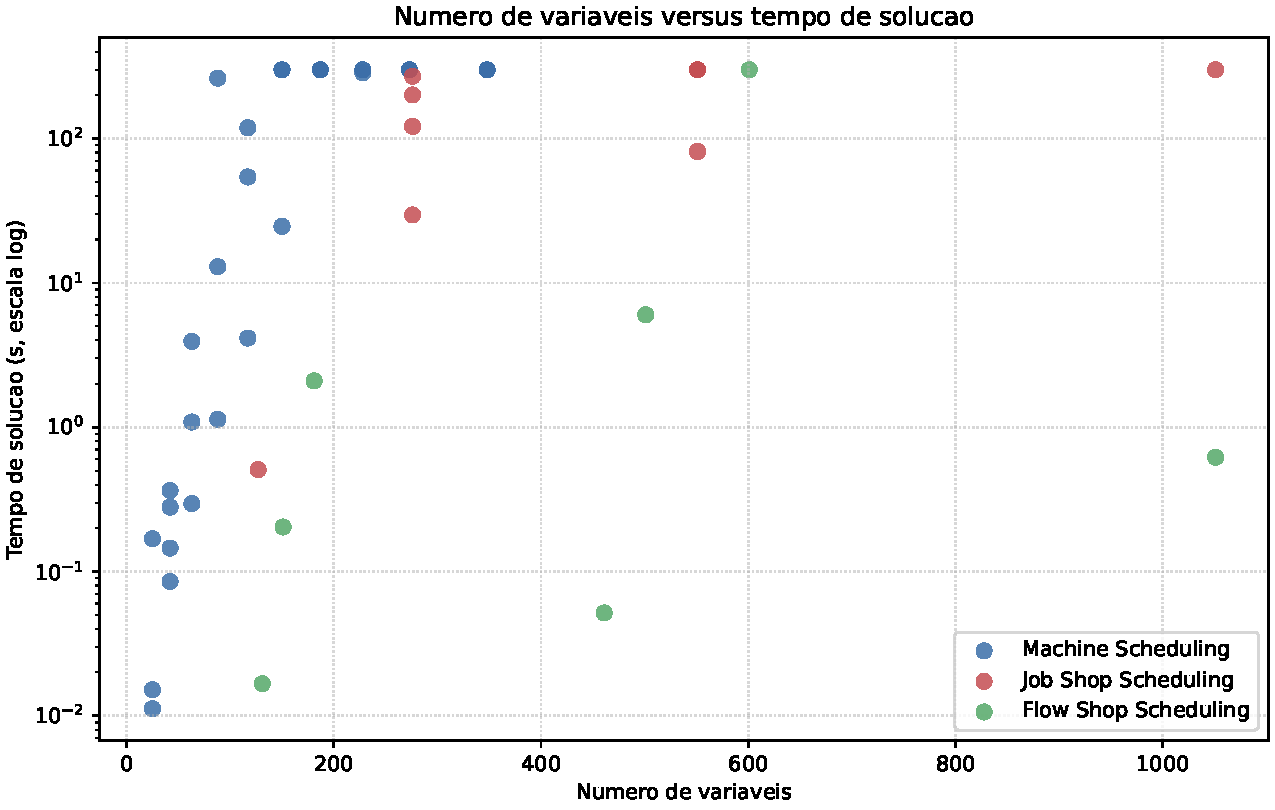
\includegraphics[width=0.90\textwidth]{variaveis_versus_tempo.pdf}
\caption{Número de variáveis versus tempo de solução.}
\label{fig:variaveis-tempo}
\end{figure}

A Figura~\ref{fig:variaveis-tempo} sugere associação entre porte do modelo e
tempo de solução, especialmente nas instâncias com maior número de variáveis.
Em Job Shop Scheduling, essa relação é acompanhada por restrições de
precedência e conflitos de máquina.

\begin{figure}[H]
\centering
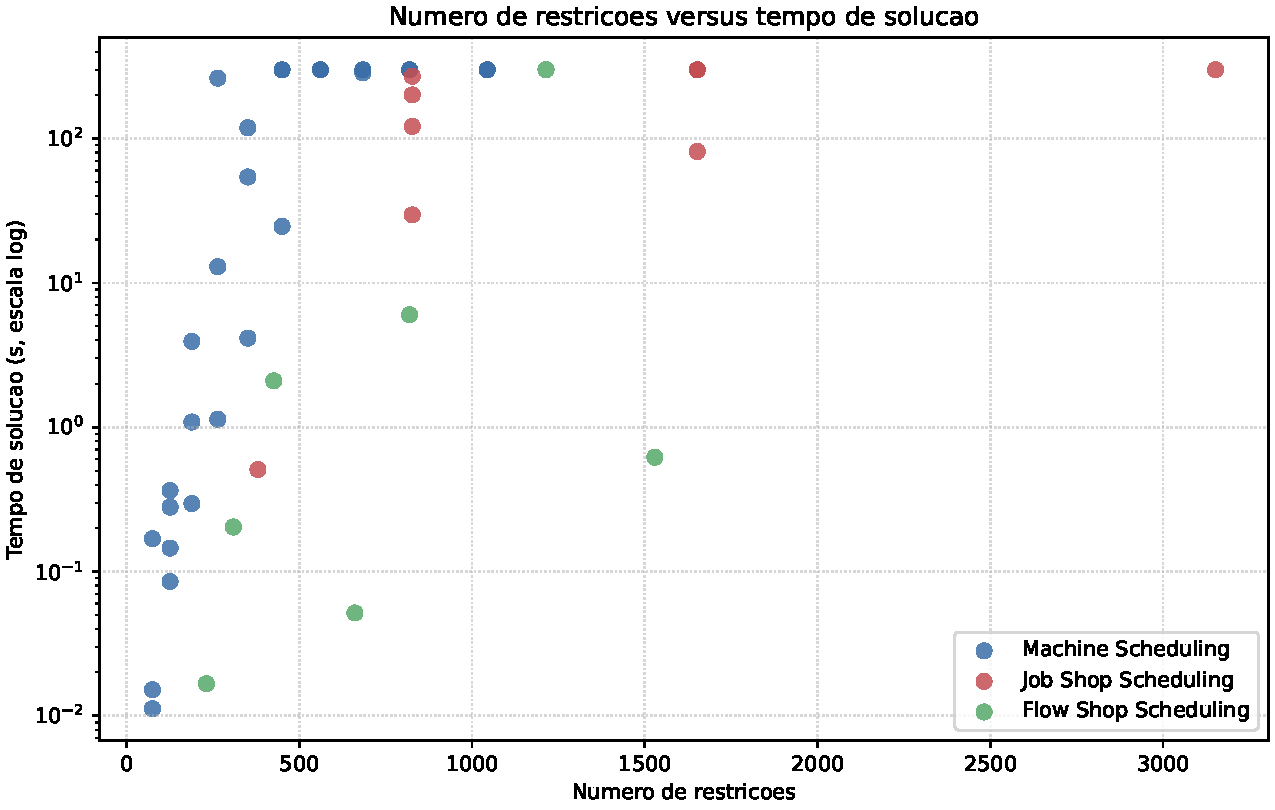
\includegraphics[width=0.90\textwidth]{restricoes_versus_tempo.pdf}
\caption{Número de restrições versus tempo de solução.}
\label{fig:restricoes-tempo}
\end{figure}

A Figura~\ref{fig:restricoes-tempo} reforça que modelos maiores tendem a
aparecer entre os casos mais custosos, embora o tempo de solução também dependa
da estrutura combinatória de cada instância.

\subsection{Flow Shop Scheduling}

Flow Shop Scheduling teve 7 instâncias analisadas, com 6 resultados ótimos e 1
interrupção por limite de tempo. O problema apresentou os menores tempos médio
e mediano entre os três conjuntos analisados.

\begin{figure}[H]
\centering
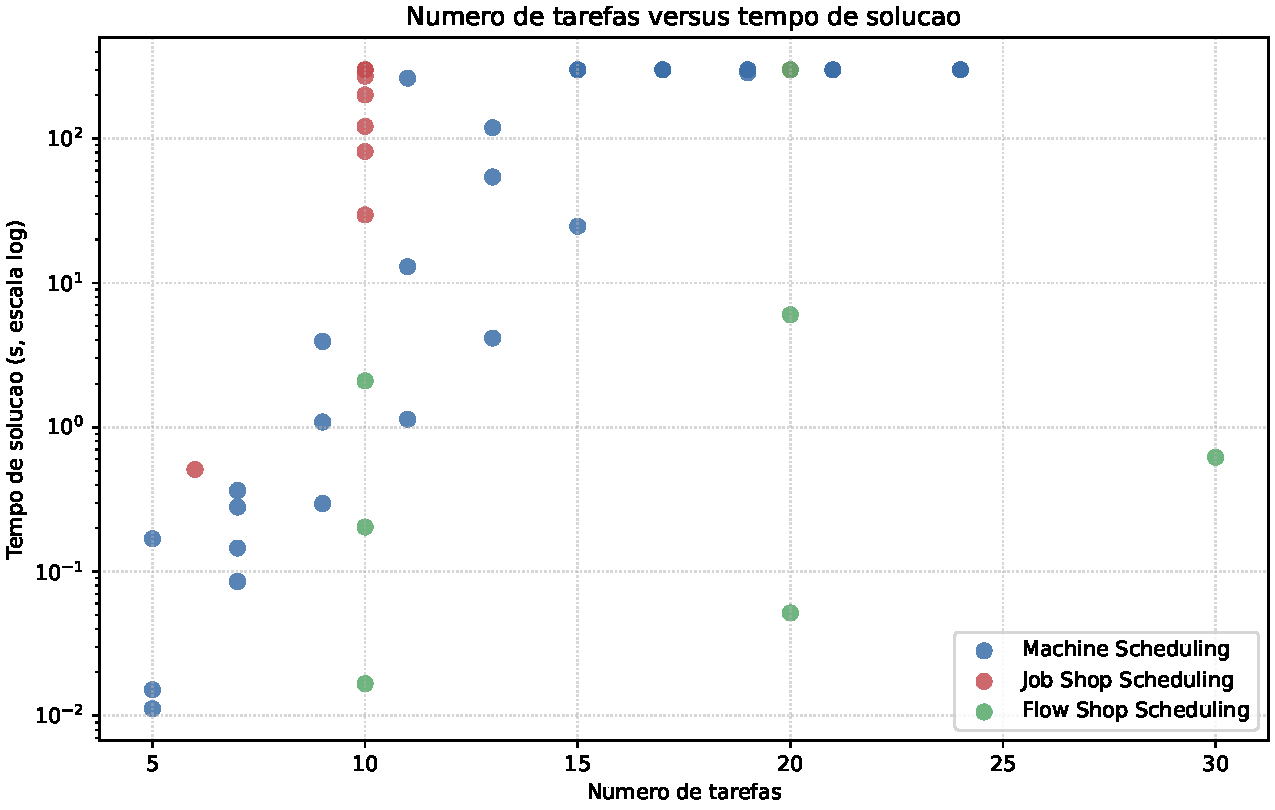
\includegraphics[width=0.90\textwidth]{tarefas_versus_tempo.pdf}
\caption{Número de tarefas versus tempo de solução.}
\label{fig:tarefas-tempo}
\end{figure}

Na Figura~\ref{fig:tarefas-tempo}, o número de tarefas não explica sozinho o
tempo de solução. Em Flow Shop Scheduling, a estrutura de sequência comum nas
máquinas contribuiu para resultados mais estáveis no conjunto observado.

\begin{figure}[H]
\centering
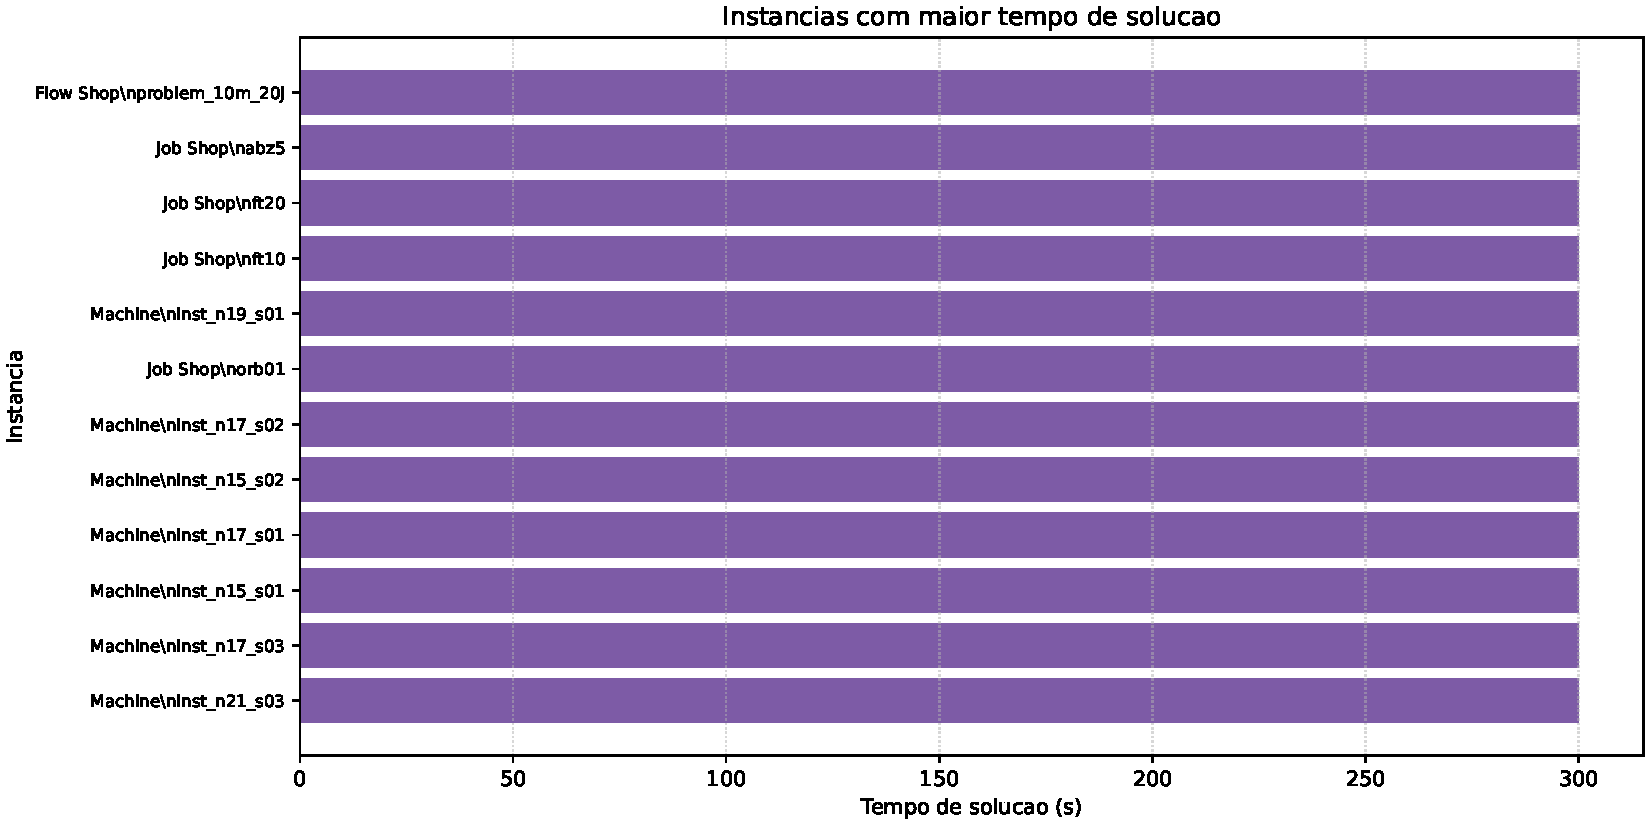
\includegraphics[width=0.90\textwidth]{instancias_maior_tempo.pdf}
\caption{Instâncias com maior tempo de solução.}
\label{fig:maior-tempo}
\end{figure}

A Figura~\ref{fig:maior-tempo} destaca as instâncias mais demoradas. A única
instância de Flow Shop Scheduling interrompida por limite de tempo aparece
entre esses casos, mas o conjunto desse problema teve desempenho geral mais
favorável.

\subsection{Tabelas específicas}

A Tabela~\ref{tab:mais-demoradas} apresenta as cinco instâncias mais demoradas
de cada problema. Os tempos próximos de 300 segundos correspondem, em geral, a
casos interrompidos pelo limite de tempo.

\begin{longtable}{llrrrrr}
\caption{Cinco instâncias mais demoradas de cada problema.}
\label{tab:mais-demoradas}\\
\toprule
Problema & Instância & Tarefas & Máq. & Oper. & Tempo (s) & Gap \\
\midrule
\endfirsthead
\toprule
Problema & Instância & Tarefas & Máq. & Oper. & Tempo (s) & Gap \\
\midrule
\endhead
Machine & \texttt{inst\_n19\_s01} & 19 & 1 & 19 & 300,019 & 0,8425 \\
Machine & \texttt{inst\_n17\_s02} & 17 & 1 & 17 & 300,018 & 0,8351 \\
Machine & \texttt{inst\_n15\_s02} & 15 & 1 & 15 & 300,017 & 0,4779 \\
Machine & \texttt{inst\_n17\_s01} & 17 & 1 & 17 & 300,017 & 0,6533 \\
Machine & \texttt{inst\_n15\_s01} & 15 & 1 & 15 & 300,015 & 0,6486 \\
Job Shop & \texttt{abz5} & 10 & 10 & 100 & 300,218 & 0,1425 \\
Job Shop & \texttt{ft20} & 20 & 5 & 100 & 300,036 & 0,6008 \\
Job Shop & \texttt{ft10} & 10 & 10 & 100 & 300,019 & 0,2157 \\
Job Shop & \texttt{orb01} & 10 & 10 & 100 & 300,019 & 0,2879 \\
Job Shop & \texttt{la02} & 10 & 5 & 50 & 270,615 & 0,0100 \\
Flow Shop & \texttt{problem\_10m\_20j} & 20 & 10 & 200 & 300,249 & 0,0241 \\
Flow Shop & \texttt{problem\_5m\_20j} & 20 & 5 & 100 & 6,014 & 0,0100 \\
Flow Shop & \texttt{problem\_8m\_10j} & 10 & 8 & 80 & 2,096 & 0,0077 \\
Flow Shop & \texttt{problem\_5m\_30j} & 30 & 5 & 150 & 0,619 & 0,0091 \\
Flow Shop & \texttt{problem\_5m\_10j} & 10 & 5 & 50 & 0,203 & 0,0046 \\
\bottomrule
\end{longtable}

A Tabela~\ref{tab:limite-tempo} lista as instâncias que atingiram limite de
tempo. A maior parte pertence a Machine Scheduling, seguida por Job Shop
Scheduling e por uma instância de Flow Shop Scheduling.

\begin{longtable}{llrrrrr}
\caption{Instâncias interrompidas pelo limite de tempo.}
\label{tab:limite-tempo}\\
\toprule
Problema & Instância & Tarefas & Máq. & Oper. & Tempo (s) & Gap \\
\midrule
\endfirsthead
\toprule
Problema & Instância & Tarefas & Máq. & Oper. & Tempo (s) & Gap \\
\midrule
\endhead
Machine & \texttt{inst\_n15\_s01} & 15 & 1 & 15 & 300,015 & 0,6486 \\
Machine & \texttt{inst\_n15\_s02} & 15 & 1 & 15 & 300,017 & 0,4779 \\
Machine & \texttt{inst\_n17\_s01} & 17 & 1 & 17 & 300,017 & 0,6533 \\
Machine & \texttt{inst\_n17\_s02} & 17 & 1 & 17 & 300,018 & 0,8351 \\
Machine & \texttt{inst\_n17\_s03} & 17 & 1 & 17 & 300,014 & 0,7035 \\
Machine & \texttt{inst\_n19\_s01} & 19 & 1 & 19 & 300,019 & 0,8425 \\
Machine & \texttt{inst\_n19\_s02} & 19 & 1 & 19 & 285,767 & 0,9712 \\
Machine & \texttt{inst\_n19\_s03} & 19 & 1 & 19 & 300,011 & 0,9229 \\
Machine & \texttt{inst\_n21\_s01} & 21 & 1 & 21 & 300,013 & 0,9083 \\
Machine & \texttt{inst\_n21\_s02} & 21 & 1 & 21 & 300,012 & 0,9755 \\
Machine & \texttt{inst\_n21\_s03} & 21 & 1 & 21 & 300,014 & 0,9189 \\
Machine & \texttt{inst\_n24\_s01} & 24 & 1 & 24 & 300,012 & 1,0000 \\
Machine & \texttt{inst\_n24\_s02} & 24 & 1 & 24 & 300,012 & 0,9847 \\
Machine & \texttt{inst\_n24\_s03} & 24 & 1 & 24 & 300,014 & 0,9629 \\
Job Shop & \texttt{abz5} & 10 & 10 & 100 & 300,218 & 0,1425 \\
Job Shop & \texttt{ft10} & 10 & 10 & 100 & 300,019 & 0,2157 \\
Job Shop & \texttt{ft20} & 20 & 5 & 100 & 300,036 & 0,6008 \\
Job Shop & \texttt{orb01} & 10 & 10 & 100 & 300,019 & 0,2879 \\
Flow Shop & \texttt{problem\_10m\_20j} & 20 & 10 & 200 & 300,249 & 0,0241 \\
\bottomrule
\end{longtable}

A Tabela~\ref{tab:maior-gap} apresenta as instâncias com maior gap. Os maiores
valores ocorreram em Machine Scheduling, principalmente nas instâncias de maior
porte.

\begin{longtable}{llrrrrr}
\caption{Instâncias com maior gap relativo por problema.}
\label{tab:maior-gap}\\
\toprule
Problema & Instância & Tarefas & Máq. & Oper. & Tempo (s) & Gap \\
\midrule
\endfirsthead
\toprule
Problema & Instância & Tarefas & Máq. & Oper. & Tempo (s) & Gap \\
\midrule
\endhead
Machine & \texttt{inst\_n24\_s01} & 24 & 1 & 24 & 300,012 & 1,0000 \\
Machine & \texttt{inst\_n24\_s02} & 24 & 1 & 24 & 300,012 & 0,9847 \\
Machine & \texttt{inst\_n21\_s02} & 21 & 1 & 21 & 300,012 & 0,9755 \\
Machine & \texttt{inst\_n19\_s02} & 19 & 1 & 19 & 285,767 & 0,9712 \\
Machine & \texttt{inst\_n24\_s03} & 24 & 1 & 24 & 300,014 & 0,9629 \\
Job Shop & \texttt{ft20} & 20 & 5 & 100 & 300,036 & 0,6008 \\
Job Shop & \texttt{orb01} & 10 & 10 & 100 & 300,019 & 0,2879 \\
Job Shop & \texttt{ft10} & 10 & 10 & 100 & 300,019 & 0,2157 \\
Job Shop & \texttt{abz5} & 10 & 10 & 100 & 300,218 & 0,1425 \\
Job Shop & \texttt{la02} & 10 & 5 & 50 & 270,615 & 0,0100 \\
Flow Shop & \texttt{problem\_10m\_20j} & 20 & 10 & 200 & 300,249 & 0,0241 \\
Flow Shop & \texttt{problem\_5m\_20j} & 20 & 5 & 100 & 6,014 & 0,0100 \\
Flow Shop & \texttt{problem\_5m\_30j} & 30 & 5 & 150 & 0,619 & 0,0091 \\
Flow Shop & \texttt{problem\_8m\_10j} & 10 & 8 & 80 & 2,096 & 0,0077 \\
Flow Shop & \texttt{problem\_5m\_10j} & 10 & 5 & 50 & 0,203 & 0,0046 \\
\bottomrule
\end{longtable}

A Tabela~\ref{tab:maior-porte} lista as instâncias de maior porte por problema.
Essas instâncias concentram os maiores números de tarefas, máquinas, operações
ou variáveis, e aparecem com frequência entre os casos de maior tempo ou maior
gap.

\begin{longtable}{llrrrrrr}
\caption{Instâncias de maior porte por problema.}
\label{tab:maior-porte}\\
\toprule
Problema & Instância & Tarefas & Máq. & Oper. & Var. & Restr. & Status \\
\midrule
\endfirsthead
\toprule
Problema & Instância & Tarefas & Máq. & Oper. & Var. & Restr. & Status \\
\midrule
\endhead
Machine & \texttt{inst\_n24\_s01} & 24 & 1 & 24 & 348 & 1044 & TIME\_LIMIT \\
Machine & \texttt{inst\_n24\_s02} & 24 & 1 & 24 & 348 & 1044 & TIME\_LIMIT \\
Machine & \texttt{inst\_n24\_s03} & 24 & 1 & 24 & 348 & 1044 & TIME\_LIMIT \\
Machine & \texttt{inst\_n21\_s01} & 21 & 1 & 21 & 273 & 819 & TIME\_LIMIT \\
Machine & \texttt{inst\_n21\_s02} & 21 & 1 & 21 & 273 & 819 & TIME\_LIMIT \\
Job Shop & \texttt{ft20} & 20 & 5 & 100 & 1051 & 3152 & TIME\_LIMIT \\
Job Shop & \texttt{abz5} & 10 & 10 & 100 & 551 & 1652 & TIME\_LIMIT \\
Job Shop & \texttt{abz6} & 10 & 10 & 100 & 551 & 1652 & OPTIMAL \\
Job Shop & \texttt{ft10} & 10 & 10 & 100 & 551 & 1652 & TIME\_LIMIT \\
Job Shop & \texttt{orb01} & 10 & 10 & 100 & 551 & 1652 & TIME\_LIMIT \\
Flow Shop & \texttt{problem\_10m\_20j} & 20 & 10 & 200 & 601 & 1214 & TIME\_LIMIT \\
Flow Shop & \texttt{problem\_5m\_30j} & 30 & 5 & 150 & 1051 & 1529 & OPTIMAL \\
Flow Shop & \texttt{problem\_5m\_20j} & 20 & 5 & 100 & 501 & 819 & OPTIMAL \\
Flow Shop & \texttt{problem\_8m\_10j} & 10 & 8 & 80 & 181 & 426 & OPTIMAL \\
Flow Shop & \texttt{problem\_3m\_20j} & 20 & 3 & 60 & 461 & 661 & OPTIMAL \\
\bottomrule
\end{longtable}

A Tabela~\ref{tab:gantt-instancias} mostra as instâncias utilizadas nos
gráficos de Gantt. Todas possuem solução primal e status ótimo nos resultados
registrados.

\begin{table}[H]
\centering
\caption{Instâncias selecionadas para os gráficos de Gantt.}
\label{tab:gantt-instancias}
\scriptsize
\begin{tabular}{llrrrrrr}
\toprule
Problema & Instância & Tarefas & Máq. & Oper. & Status & Tempo (s) & Gap \\
\midrule
Machine & \texttt{inst\_n05\_s01} & 5 & 1 & 5 & OPTIMAL & 0,015 & 0,0000 \\
Job Shop & \texttt{ft06} & 6 & 6 & 36 & OPTIMAL & 0,509 & 0,0000 \\
Flow Shop & \texttt{problem\_3m\_10j} & 10 & 3 & 30 & OPTIMAL & 0,017 & 0,0000 \\
\bottomrule
\end{tabular}
\end{table}

Não houve instâncias com erro nos resultados consolidados, conforme indicado na
Tabela~\ref{tab:geral} e na tabela específica de erros gerada pelo script de
resultados.

\subsection{Gráficos de Gantt}

\begin{figure}[H]
\centering
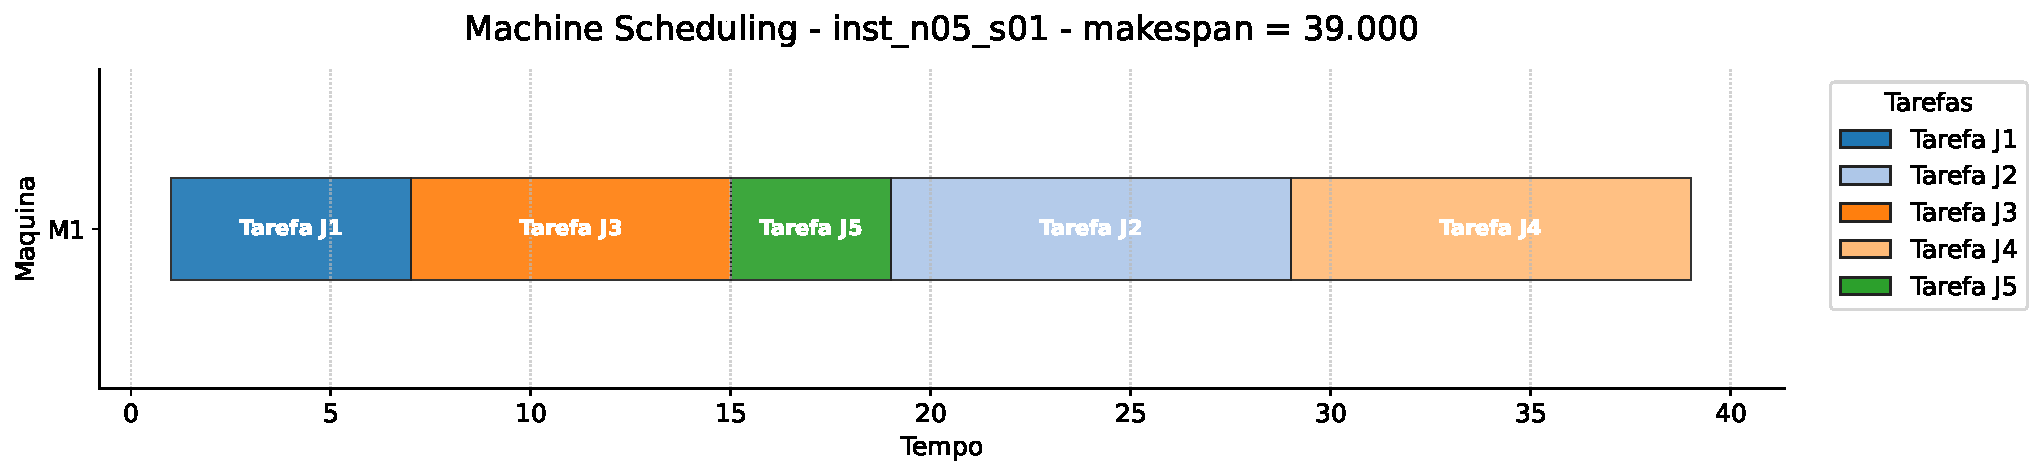
\includegraphics[width=0.92\textwidth]{gantt_machine_inst_n05_s01_estilo_professor.pdf}
\caption{Gantt de Machine Scheduling para a programação das tarefas da instância \texttt{inst\_n05\_s01}.}
\label{fig:gantt-machine}
\end{figure}

Na Figura~\ref{fig:gantt-machine}, todas as tarefas são processadas em uma
única máquina. A própria máquina determina o makespan da programação.

\begin{figure}[H]
\centering
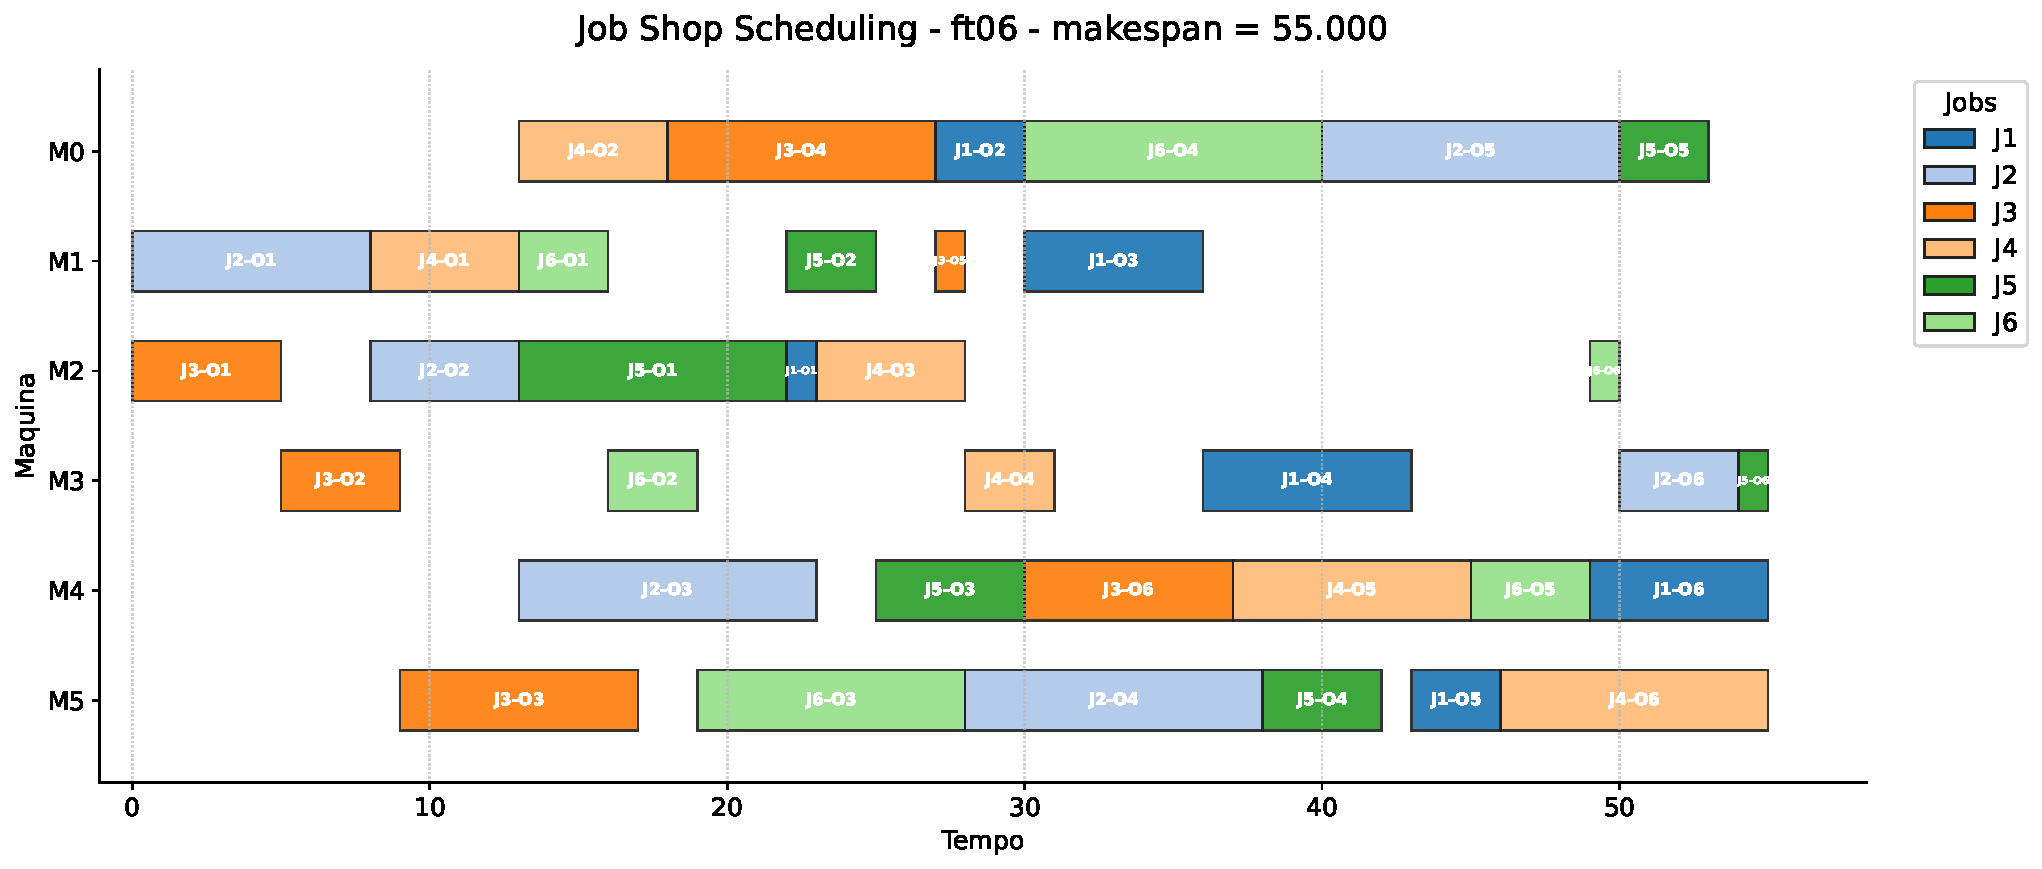
\includegraphics[width=0.94\textwidth]{gantt_job_shop_ft06_estilo_professor.pdf}
\caption{Gantt de Job Shop Scheduling para a programação das operações da instância \texttt{ft06}.}
\label{fig:gantt-job}
\end{figure}

A Figura~\ref{fig:gantt-job} mostra a interação entre precedências dos jobs e
conflitos por máquina. As esperas entre operações decorrem da necessidade de
respeitar simultaneamente a ordem tecnológica e a disponibilidade das máquinas.

\begin{figure}[H]
\centering
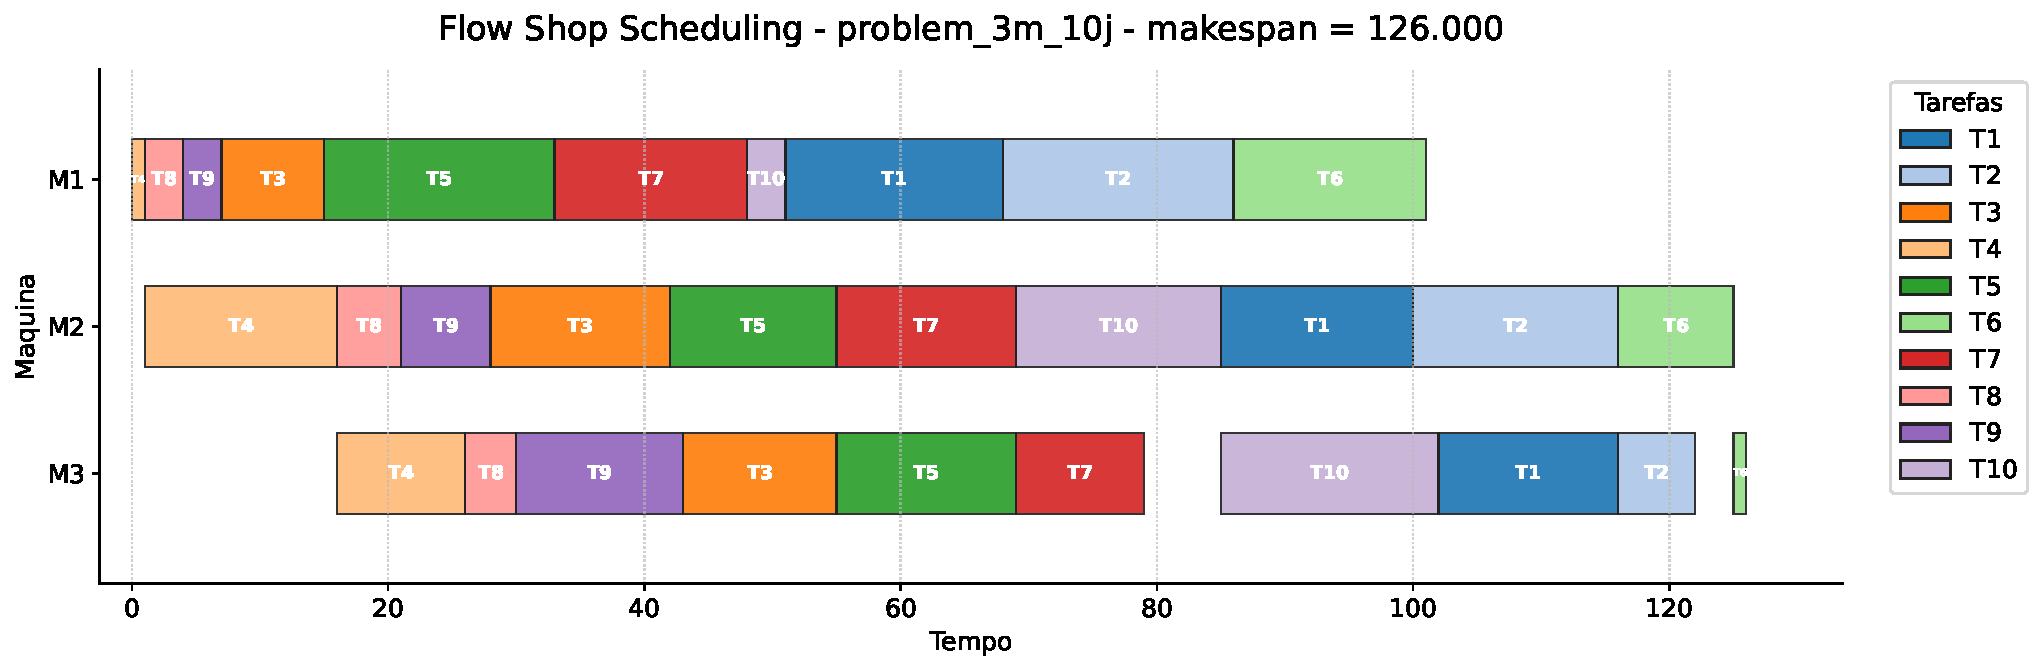
\includegraphics[width=0.94\textwidth]{gantt_flow_shop_problem_3m_10j_estilo_professor.pdf}
\caption{Gantt de Flow Shop Scheduling para a programação das tarefas nas máquinas da instância \texttt{problem\_3m\_10j}.}
\label{fig:gantt-flow}
\end{figure}

A Figura~\ref{fig:gantt-flow} evidencia o fluxo das tarefas pela sequência
comum de máquinas. A programação apresenta tempos ociosos resultantes do
encadeamento entre estágios e da carga desigual entre máquinas.

\subsection{Dashboard comparativo}

\begin{landscape}
\begin{figure}[p]
\centering
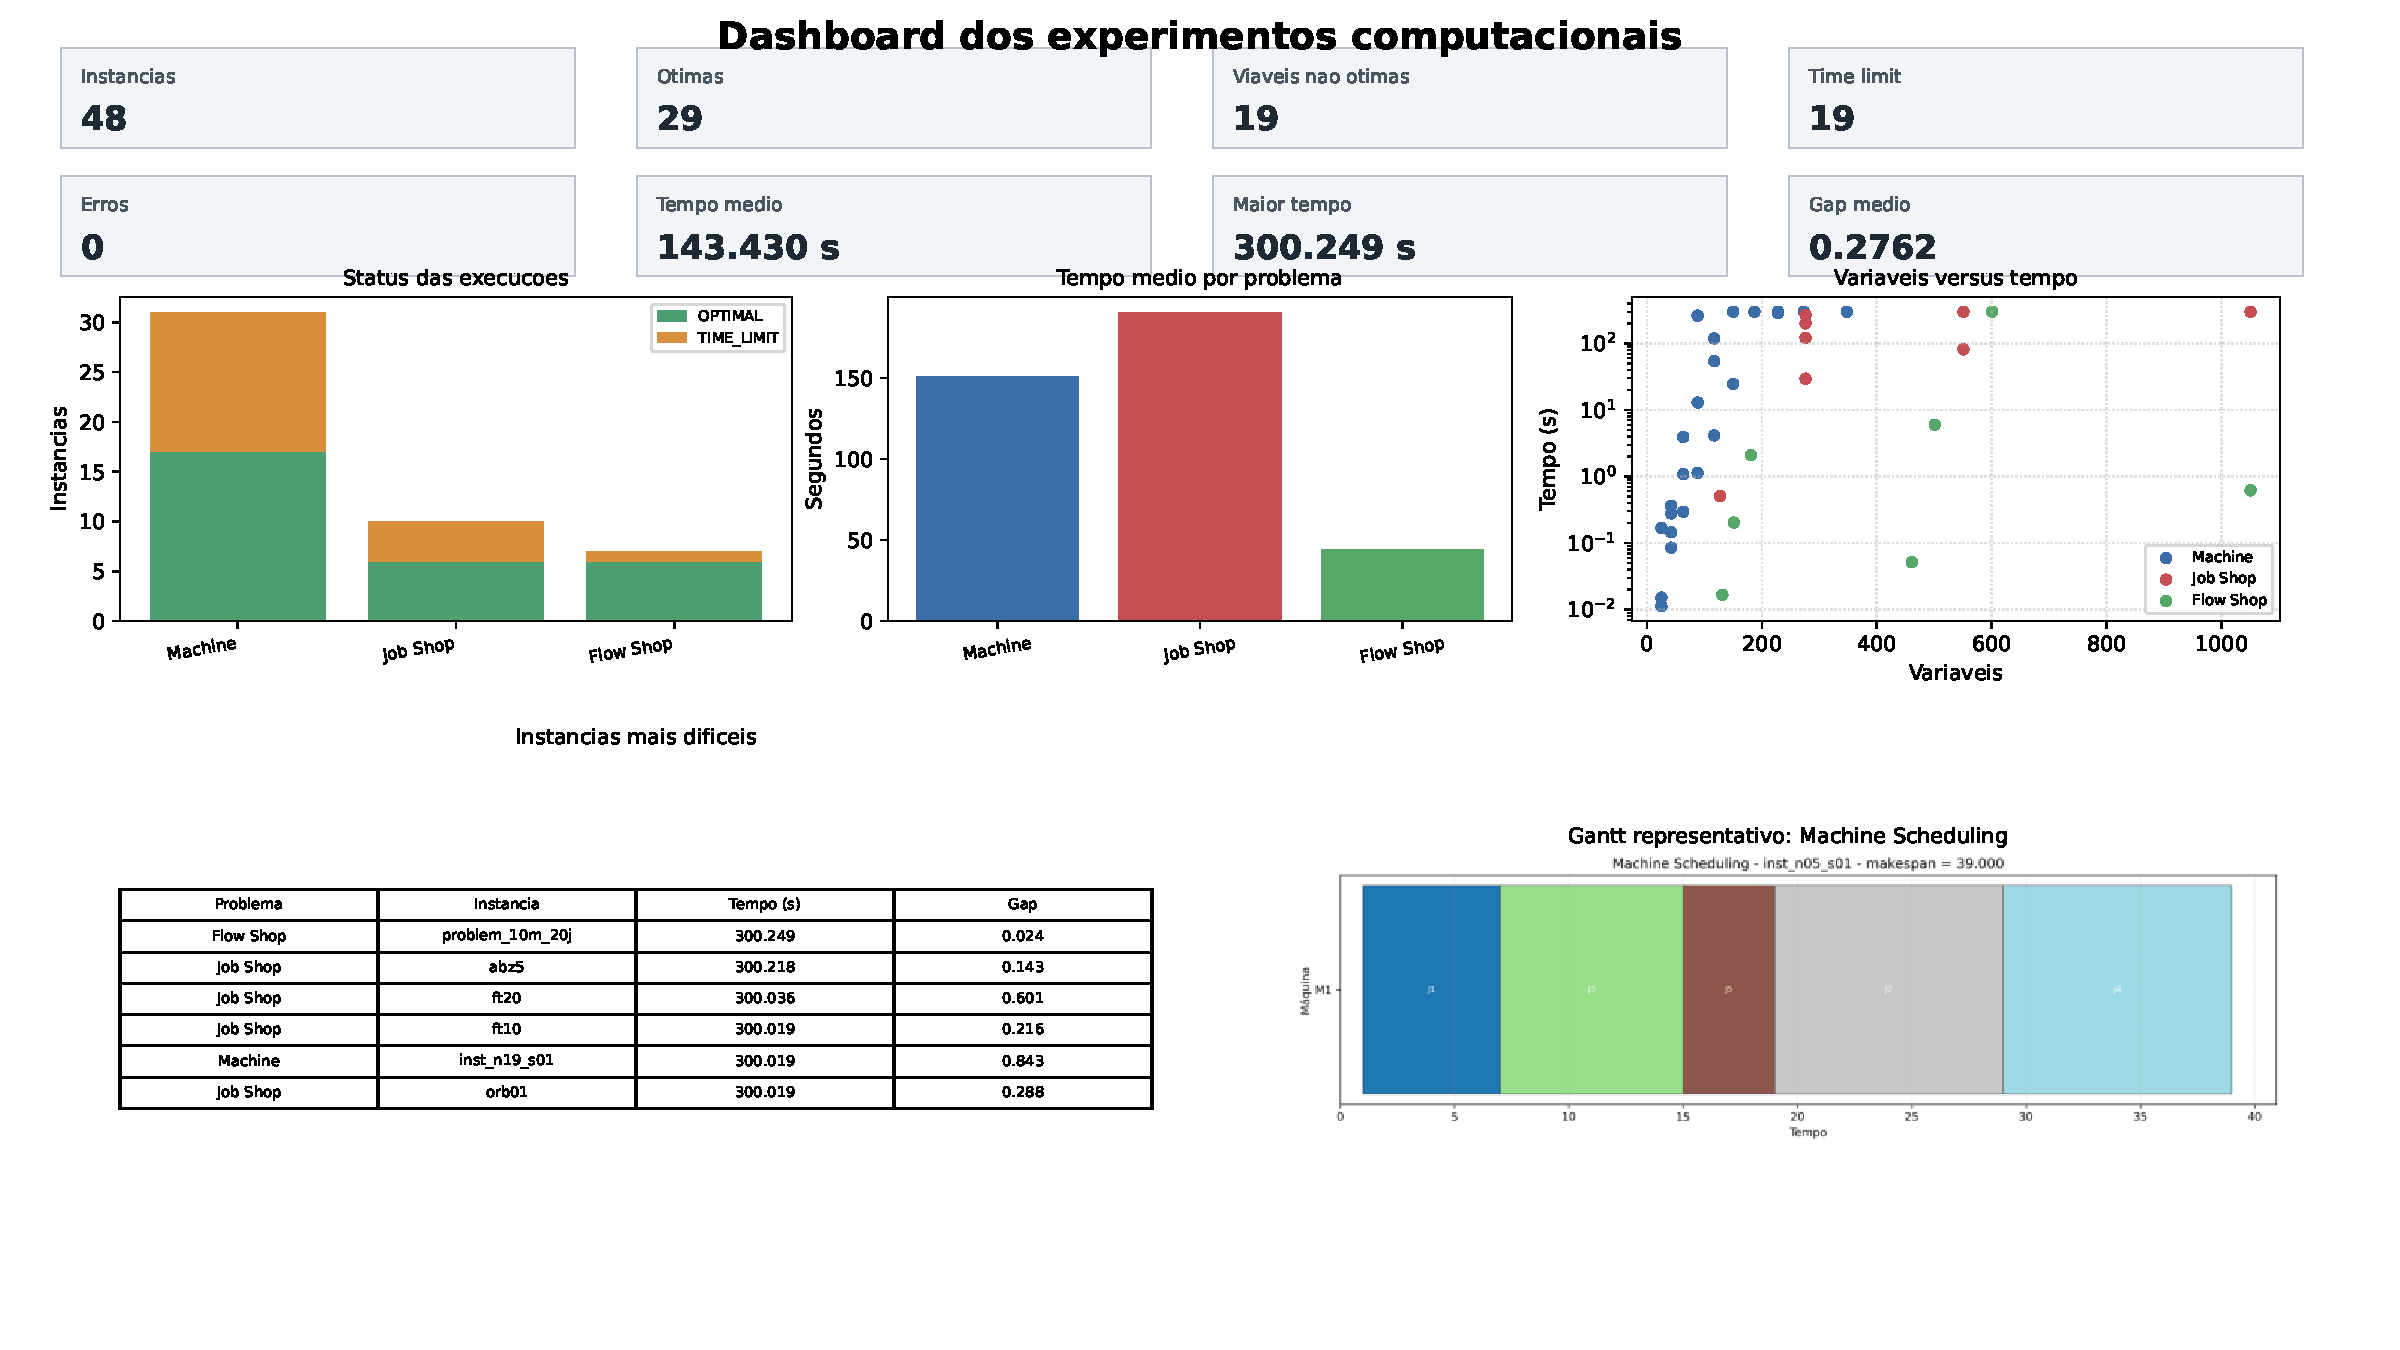
\includegraphics[width=0.96\linewidth,height=0.86\textheight,keepaspectratio]{dashboard_resultados.pdf}
\caption{Dashboard comparativo dos resultados computacionais.}
\label{fig:dashboard}
\end{figure}
\end{landscape}

O dashboard da Figura~\ref{fig:dashboard} consolida os principais indicadores
do experimento, incluindo status das execuções, tempos médios por problema,
relações entre porte e tempo de solução e instâncias de maior dificuldade. A
visualização reforça a diferença de comportamento entre os três problemas.

\section{Discussão dos resultados}

Esta discussão utiliza exclusivamente os dados registrados em
\texttt{resultados\_completos.csv}, as tabelas e gráficos gerais gerados a partir
desse arquivo, o dashboard estático e os dados detalhados dos gráficos de Gantt.
Assim, as interpretações apresentadas estão restritas ao conjunto de instâncias
executado, às formulações implementadas e à configuração computacional adotada:
limite de tempo de 300 segundos por instância e tolerância relativa de gap de
1\%.

\subsection{Resultados observados}

Foram analisadas 48 instâncias no total: 31 de Machine Scheduling, 10 de Job
Shop Scheduling e 7 de Flow Shop Scheduling. O HiGHS encontrou solução primal
viável em todas as instâncias registradas, e não houve erros de execução nos
resultados consolidados.

O problema com maior proporção de soluções ótimas foi o Flow Shop Scheduling,
com 6 soluções ótimas em 7 instâncias, correspondendo a aproximadamente 85,7\%
do conjunto desse problema. O Job Shop Scheduling apresentou 6 soluções ótimas
em 10 instâncias, isto é, 60,0\%. O Machine Scheduling teve 17 soluções ótimas
em 31 instâncias, aproximadamente 54,8\%. Portanto, embora Machine Scheduling
tenha apresentado a maior quantidade absoluta de soluções ótimas, Flow Shop
Scheduling apresentou a maior proporção de instâncias resolvidas dentro da
tolerância de otimalidade configurada.

Em relação ao tempo de solução, o Job Shop Scheduling apresentou o maior tempo
médio, 190,464 segundos, e também o maior tempo mediano, 235,695 segundos. O
Machine Scheduling teve tempo médio de 150,670 segundos e mediana de 119,012
segundos. O Flow Shop Scheduling apresentou o menor tempo médio, 44,178
segundos, e a menor mediana, 0,619 segundo. Esses valores indicam que, no
conjunto de dados considerado, Job Shop foi o problema com comportamento mais
custoso em termos de tempo central típico, enquanto Machine Scheduling concentrou
maior número absoluto de interrupções por limite de tempo.

As instâncias que atingiram o limite de tempo foram 14 em Machine Scheduling, 4
em Job Shop Scheduling e 1 em Flow Shop Scheduling. Em Machine Scheduling, todas
as interrupções ocorreram em instâncias com 15 ou mais tarefas. Em Job Shop, as
instâncias interrompidas foram \texttt{abz5}, \texttt{ft10}, \texttt{ft20} e
\texttt{orb01}. Em Flow Shop, apenas \texttt{problem\_10m\_20j} atingiu o limite
de tempo. O dashboard e a tabela de instâncias com maior tempo mostram que
essas instâncias aparecem entre os casos mais custosos do experimento.

O comportamento do gap também variou substancialmente entre os problemas. O gap
médio geral foi 0,3841 em Machine Scheduling, 0,1297 em Job Shop Scheduling e
0,0079 em Flow Shop Scheduling. Considerando apenas as soluções não ótimas, os
gaps médios foram 0,8432 para Machine Scheduling, 0,3118 para Job Shop
Scheduling e 0,0241 para Flow Shop Scheduling. O maior gap registrado ocorreu em
Machine Scheduling, com valor aproximadamente igual a 1,0000. Em Job Shop, o
maior gap foi 0,6008, observado em \texttt{ft20}. Em Flow Shop, o maior gap foi
0,0241, correspondente à única instância interrompida pelo limite de tempo.

\subsection{Possíveis explicações}

Os resultados sugerem que a dificuldade computacional está associada à
combinação entre tamanho da instância, número de variáveis, número de restrições
e estrutura combinatória do modelo. Essa relação aparece nos gráficos de
tarefas versus tempo, variáveis versus tempo e restrições versus tempo, embora
não seja perfeitamente determinística.

No Machine Scheduling, todas as instâncias possuem apenas uma máquina, mas o
modelo utiliza variáveis binárias associadas a pares de tarefas. A média de
variáveis foi 148,548 e a média de restrições foi 445,645, com máximos de 348
variáveis e 1044 restrições. As instâncias de maior porte desse problema,
especialmente as com 21 e 24 tarefas, aparecem entre as maiores em número de
variáveis, restrições e gap. Uma explicação plausível é que o crescimento
combinatório das decisões de sequenciamento dificulta o fechamento do gap, mesmo
em máquina única.

No Job Shop Scheduling, o número médio de tarefas foi 10,6 e o número médio de
máquinas foi 7,1. A média de variáveis foi 448,6 e a média de restrições foi
1344,8, superiores às médias de Machine Scheduling. O maior modelo de Job Shop
registrado teve 1051 variáveis e 3152 restrições. Como o Job Shop combina
precedências tecnológicas por job com conflitos de capacidade em várias
máquinas, é razoável interpretar que a estrutura disjuntiva do modelo contribuiu
para os tempos elevados. Essa interpretação é compatível com o fato de o Job
Shop ter apresentado o maior tempo médio e mediano.

No Flow Shop Scheduling, a formulação posicional explorou a existência de uma
sequência comum de jobs nas máquinas. Apesar de o conjunto incluir instâncias
com até 30 tarefas e 10 máquinas, o problema apresentou a menor média de tempo e
a maior proporção de soluções ótimas. A média de variáveis foi 439,571 e a média
de restrições foi 741,286. Assim, embora os modelos de Flow Shop não sejam
pequenos em número de variáveis, a estrutura regular da sequência comum pode ter
favorecido o desempenho observado do HiGHS neste conjunto específico.

O número de máquinas também afeta os problemas de maneiras distintas. Em Machine
Scheduling ele é constante e igual a 1, logo a dificuldade observada está ligada
principalmente ao número de tarefas e às disjunções entre elas. Em Job Shop, o
número de máquinas aumenta a quantidade de conflitos de capacidade entre
operações. Em Flow Shop, mais máquinas aumentam a dimensão do modelo e a cadeia
de precedências, mas preservam a ordem comum das tarefas, o que pode explicar
por que instâncias de Flow Shop com várias máquinas ainda foram resolvidas com
mais estabilidade do que parte das instâncias de Job Shop.

\subsection{Análise dos Gantts}

Os gráficos de Gantt foram gerados para três instâncias representativas:
\texttt{inst\_n05\_s01} em Machine Scheduling, \texttt{ft06} em Job Shop
Scheduling e \texttt{problem\_3m\_10j} em Flow Shop Scheduling. Essas três
soluções foram resolvidas novamente apenas para recuperar os horários detalhados
de início e término, e as validações estruturais não indicaram violações de
precedência, duração, sobreposição ou makespan.

No Gantt de Machine Scheduling, a instância possui 5 tarefas e uma única
máquina. O makespan da programação detalhada foi 39,0. A soma dos tempos de
processamento foi 38,0, e a máquina ficou ociosa por 1,0 unidade de tempo quando
se considera o intervalo entre o tempo zero e o makespan. No intervalo efetivo
entre a primeira tarefa e a última conclusão, não houve ociosidade interna. Como
há apenas uma máquina, ela concentra toda a carga e determina diretamente o
makespan. O gráfico evidencia uma sequência compacta de tarefas após o início
da primeira operação.

No Gantt de Job Shop, a instância \texttt{ft06} possui 6 jobs, 6 máquinas e 36
operações, com makespan aproximadamente igual a 55,0. Todas as operações
esperadas estão presentes. As precedências de cada job foram respeitadas, mas
existem esperas entre operações: foram observados 30 intervalos entre operações
consecutivas de jobs, dos quais 14 tiveram espera positiva, com soma total de
esperas igual a 53,0 e maior espera igual a 8,0. Essa característica é coerente
com o Job Shop, no qual uma operação pode precisar aguardar a liberação da
máquina seguinte. Pelos dados do Gantt, as máquinas M5, M0 e M4 apresentaram
altas cargas de processamento, com 43,0, 40,0 e 40,0 unidades, respectivamente.
A máquina M5 teve a menor folga em relação ao makespan, 12,0 unidades, o que
sugere papel relevante na formação do caminho crítico da solução observada. As
máquinas M2 e M3 apresentaram maiores períodos ociosos dentro de suas janelas de
atividade, indicando que nem todas as máquinas foram igualmente pressionadas.

No Gantt de Flow Shop, a instância \texttt{problem\_3m\_10j} possui 10 tarefas e
3 máquinas, com makespan 126,0. A sequência encontrada foi
\texttt{J4 -> J8 -> J9 -> J3 -> J5 -> J7 -> J10 -> J1 -> J2 -> J6}. O fluxo das
tarefas respeita a ordem M1, M2 e M3. As cargas totais por máquina foram 101,0
em M1, 124,0 em M2 e 101,0 em M3. A máquina M2 foi a mais carregada e terminou
em 125,0, muito próxima do makespan, o que sugere que ela atuou como gargalo
principal nesta programação. A máquina M3 iniciou apenas no tempo 16,0 e teve
ociosidade interna de 9,0 unidades dentro de sua janela de atividade, além de
receber tarefas condicionadas pela conclusão em M2. Foram observadas esperas
entre máquinas em 13 dos 20 intervalos analisados, com soma total de 129,0 e
maior espera igual a 18,0. Esse comportamento é compatível com o fluxo em série:
mesmo com sequência comum, as máquinas finais podem acumular esperas decorrentes
do desalinhamento entre tempos de processamento nas etapas anteriores.

\subsection{Desempenho do HiGHS e limites da configuração}

O HiGHS foi capaz de encontrar soluções viáveis para todas as 48 instâncias
registradas. Esse é um resultado relevante, pois mesmo as instâncias
interrompidas por tempo possuem ponto primal viável. Por outro lado, a
configuração de 300 segundos e gap relativo de 1\% não foi suficiente para
encerrar todas as instâncias dentro da tolerância estabelecida. O efeito dessa
configuração é visível principalmente em Machine Scheduling e Job Shop
Scheduling, que concentraram a maior parte dos limites de tempo e dos gaps mais
altos.

Também é importante observar que o status \texttt{OPTIMAL} deve ser interpretado
dentro da tolerância configurada. Algumas instâncias com status ótimo possuem
gap positivo menor que 1\%, o que indica otimalidade de acordo com o critério de
parada adotado. Portanto, a comparação entre problemas deve considerar não
apenas o status final, mas também o gap, o tempo consumido e o tamanho do modelo.

\subsection{Limitações do experimento}

As conclusões são limitadas ao conjunto de instâncias analisado. Os tamanhos dos
conjuntos não são iguais: foram 31 instâncias de Machine Scheduling, 10 de Job
Shop Scheduling e 7 de Flow Shop Scheduling. Assim, médias e proporções devem
ser interpretadas com cautela, principalmente no Flow Shop, que possui menor
número de observações.

Outra limitação é que as formulações utilizadas são modelos MILP diretos. Em
Machine Scheduling e Job Shop, as formulações dependem de restrições
disjuntivas e variáveis binárias de ordenação, que podem produzir relaxações
lineares difíceis para o solver. No Flow Shop, a formulação posicional pareceu
mais favorável nos dados observados, mas isso não implica superioridade geral do
problema ou da formulação em outros conjuntos de instâncias.

Por fim, os resultados consolidados armazenam métricas agregadas, mas não
armazenam as programações completas de todas as soluções. Por isso, a validação
estrutural detalhada foi realizada apenas para as três instâncias selecionadas
para os gráficos de Gantt. Para análises futuras, seria recomendável registrar
também os horários de início e término de todas as operações, permitindo validar
e visualizar qualquer solução sem necessidade de nova execução do modelo.


\section{Conclusão}

Este trabalho analisou três problemas clássicos de escalonamento: Machine
Scheduling, Job Shop Scheduling e Flow Shop Scheduling. As formulações foram
implementadas em Julia, com JuMP e o solver HiGHS, e avaliadas sobre 48
instâncias registradas nos arquivos de resultados: 31 de Machine Scheduling, 10
de Job Shop Scheduling e 7 de Flow Shop Scheduling. No conjunto consolidado,
foram obtidos 29 resultados com status ótimo, distribuídos entre os três
problemas, sem registros de erro de execução nos resultados computacionais
consolidados.

Os resultados indicaram comportamentos distintos entre os problemas. O Flow Shop
Scheduling apresentou a maior proporção de soluções ótimas, com 6 instâncias
ótimas em 7, além dos menores tempos médio e mediano. O Job Shop Scheduling
apresentou os maiores tempos médio e mediano, o que evidencia maior dificuldade
computacional no comportamento central observado. O Machine Scheduling, embora
tenha apenas uma máquina nas instâncias analisadas, concentrou a maior
quantidade absoluta de interrupções por limite de tempo e os maiores gaps,
especialmente nas instâncias com maior número de tarefas. Assim, considerando
conjuntamente tempo, gap e limites de tempo, os resultados apontam maior
dificuldade prática para Machine Scheduling no fechamento da otimalidade e para
Job Shop Scheduling no esforço computacional típico.

Os gráficos de Gantt complementaram a análise agregada ao mostrar a estrutura
das soluções selecionadas. Em Machine Scheduling, a programação da instância
\texttt{inst\_n05\_s01} concentrou toda a carga em uma única máquina, que
determinou diretamente o makespan. Em Job Shop Scheduling, a instância
\texttt{ft06} evidenciou o efeito das precedências entre operações e das esperas
causadas por conflitos de máquina, com algumas máquinas atuando como gargalos
mais relevantes. Em Flow Shop Scheduling, a instância
\texttt{problem\_3m\_10j} mostrou o fluxo das tarefas pela sequência comum de
máquinas, com formação de gargalo na máquina de maior carga e presença de
tempos ociosos decorrentes do encadeamento entre estágios.

A configuração adotada, com limite de tempo de 300 segundos e gap relativo de
1\%, foi adequada para obter soluções viáveis em todas as instâncias registradas
e para resolver parte expressiva do conjunto até a otimalidade segundo o
critério do solver. Contudo, essa configuração não foi suficiente para fechar o
gap em todas as instâncias, principalmente em Machine Scheduling e Job Shop
Scheduling. A interpretação dos resultados deve considerar essa limitação, bem
como o fato de que os conjuntos possuem tamanhos diferentes e que os resultados
dependem das formulações MILP diretas utilizadas.

Como trabalhos futuros, recomenda-se avaliar formulações alternativas,
estratégias de fortalecimento das restrições, diferentes valores de Big-M,
heurísticas de geração de soluções iniciais e outros limites de tempo ou
tolerâncias de gap. Também seria útil armazenar os horários completos de início
e término para todas as instâncias, permitindo validações estruturais e gráficos
de Gantt sem necessidade de nova resolução dos modelos. Essas extensões
permitiriam uma comparação mais ampla entre formulações e uma análise mais
detalhada do comportamento computacional dos três problemas.


\end{document}
